\documentclass[../main.tex]{subfiles}
\begin{document}

\section{Environmental Setup}
\label{sec:environmental_setup}

Our experiments were conducted on a computer featuring an Intel i5-12600K CPU paired with an NVIDIA GeForce RTX 3060 GPU (12 GB of VRAM) to perform inference for the end-to-end ReID system. Each camera node in the system was equipped with a lightweight, cost-effective device configured with a single-core CPU operating at 3.5 GHz and 512MB of RAM.

\begin{table}[h]
\centering
\caption{Hardware setup on the server and the edge device}
\label{tab:hardware_setup}
\begin{tabular}{|p{3.5cm}|p{5cm}|p{5cm}|}
\hline
\textbf{Component} & \textbf{Edge Device} & \textbf{Server} \\
\hline
\textbf{CPU} & 1-core CPU 3.5 GHz & Intel i5 12600K \\
\hline
\textbf{GPU} & None & RTX 3060 12GB \\
\hline
\textbf{RAM} & 512MB & 32GB \\
\hline
\end{tabular}
\end{table}

\section{Dataset}
\label{sec:dataset}
\subsection{P-DESTRE}

The P-DESTRE (Pedestrian Detection, Tracking, Re-Identification and Search from Aerial Devices) dataset \cite{kumar2020pdestrefullyannotateddataset} is a novel, fully annotated, UAV-based dataset. It addresses limitations in existing visual surveillance datasets by providing consistent identity (ID) annotations across multiple days, making it uniquely suitable for the challenging problem of person search, where clothing appearance is unreliable for identification. This collaborative effort from researchers in Portugal and India also supports research in pedestrian detection, tracking, re-identification, soft biometrics, and action recognition.

\begin{figure}[htbp]
    \centering
    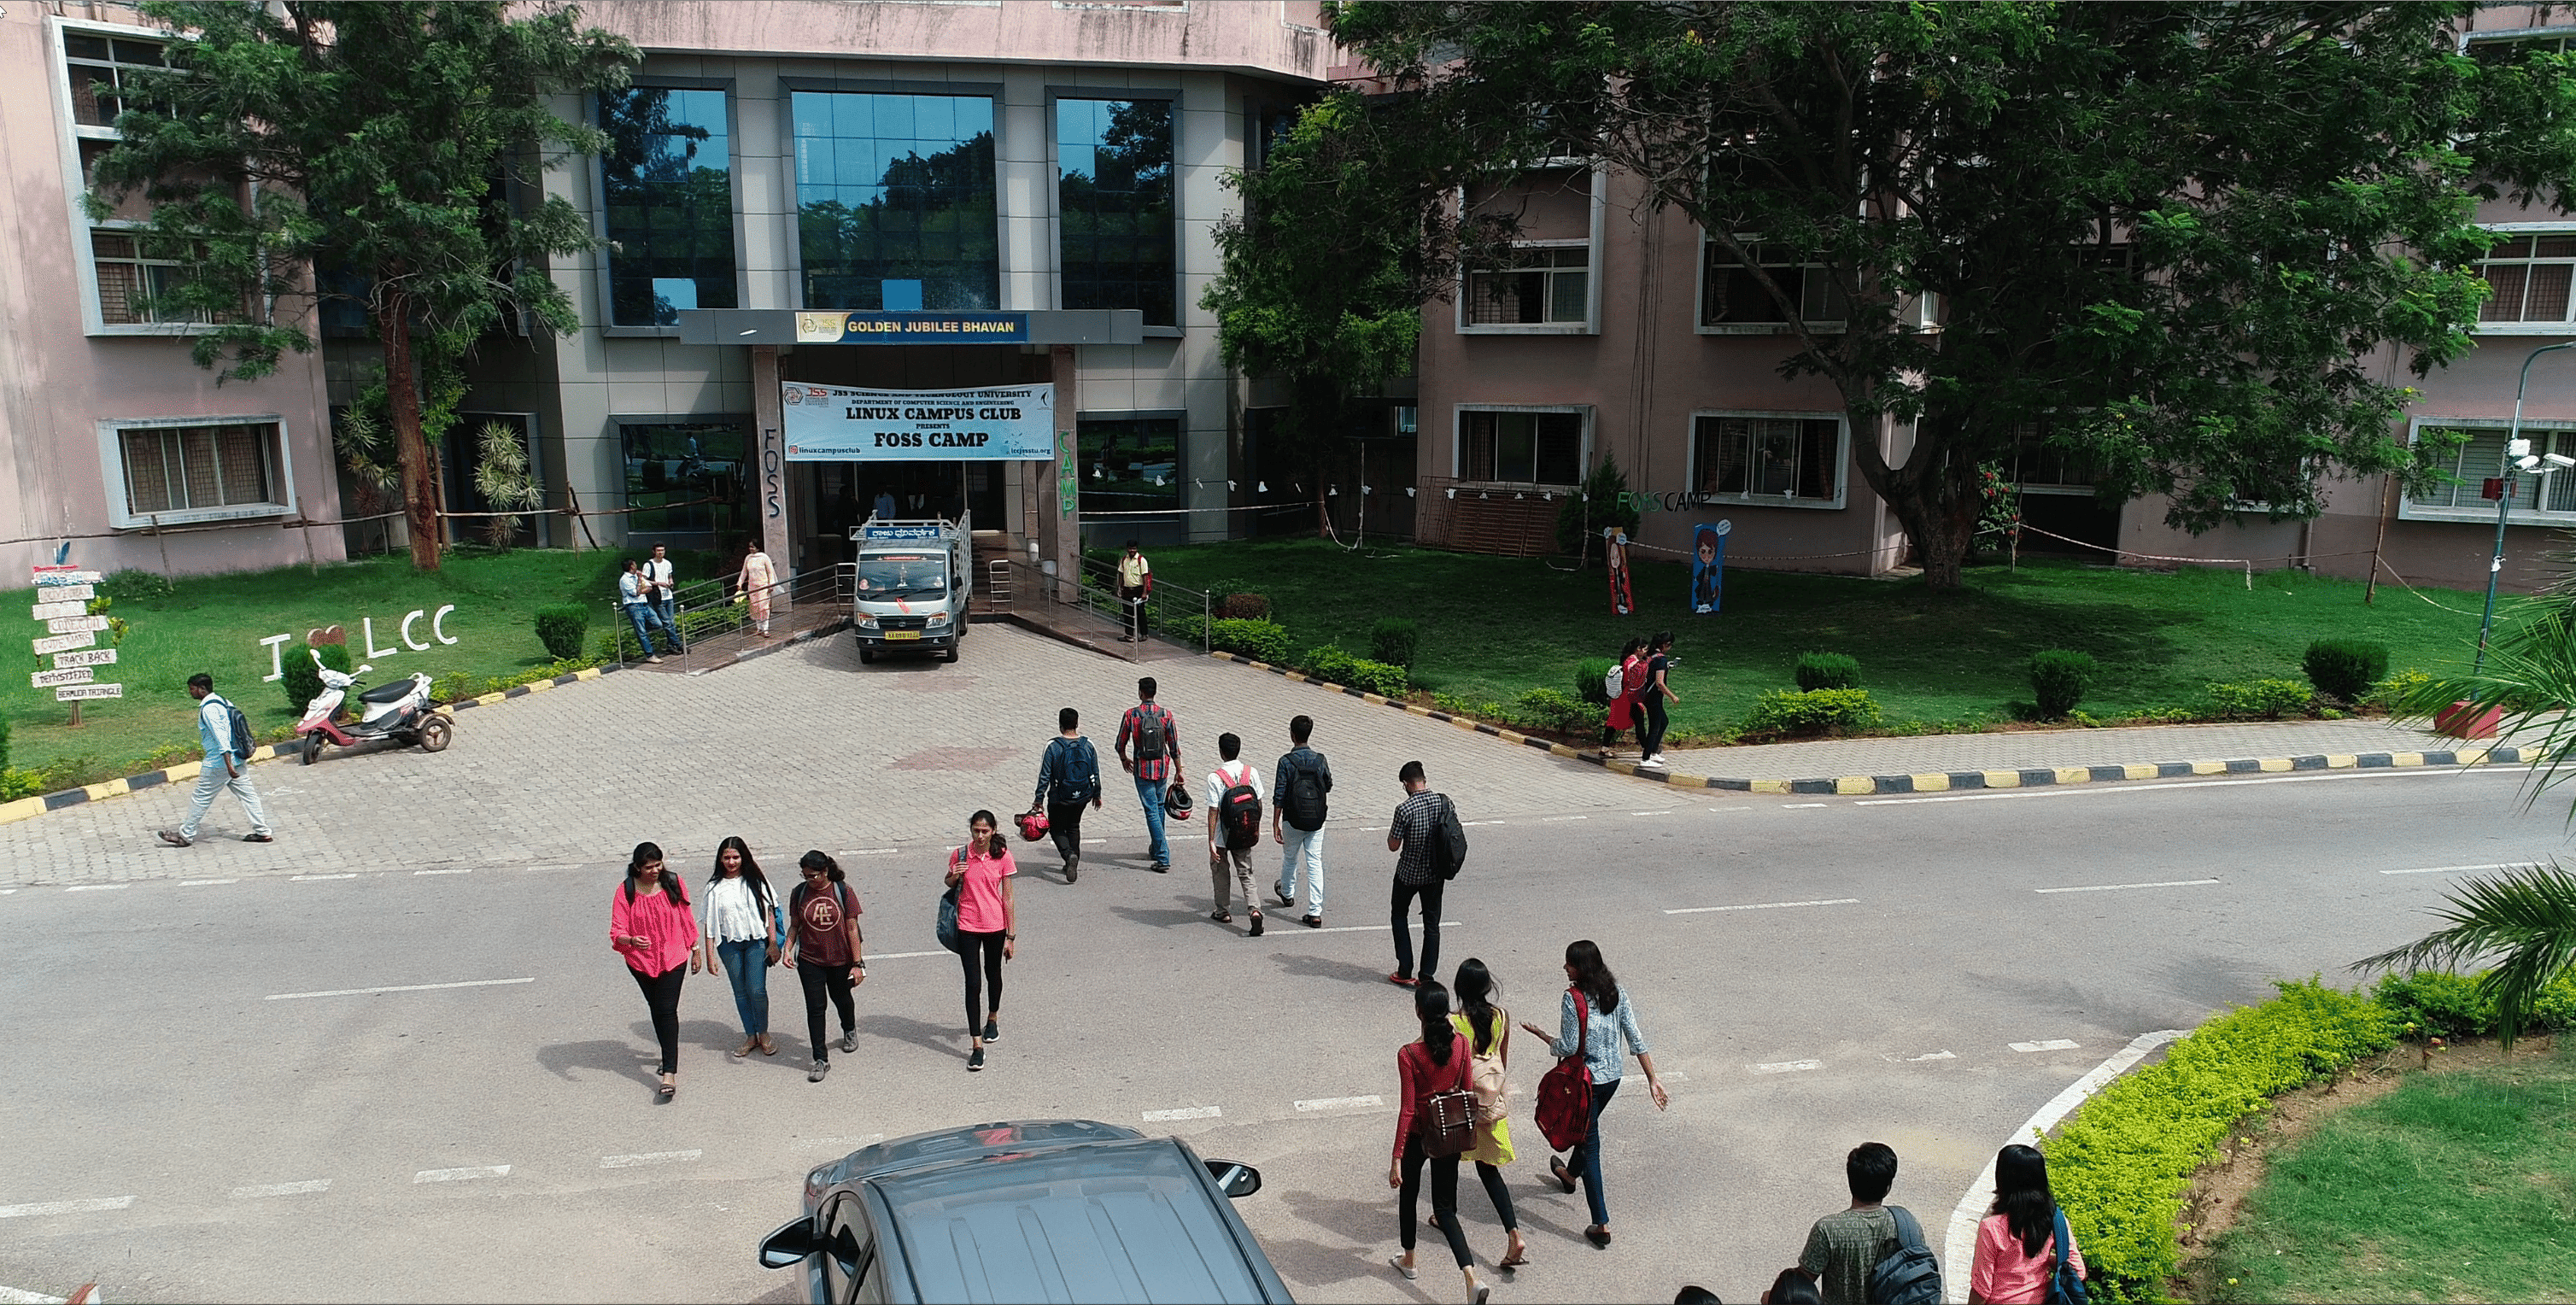
\includegraphics[width=1\textwidth]{Figure/pdestre.png}
    \caption{Sample frame from the P-DESTRE dataset showing aerial view of pedestrians captured by UAV over university campus in Portugal}
    \label{fig:pdestre_overview}
\end{figure}

Data was collected using DJI Phantom 4 drones, operated by human controllers, over university campuses in Portugal and India. The acquisition simulated everyday crowded outdoor urban environments (as shown in Figure \ref{fig:pdestre_overview}). Volunteers participated willingly, ignoring the UAVs which flew at altitudes between 5.5 and 6.7 meters with camera pitch angles from 45$^\circ$ to 90$^\circ$. Videos were recorded at 30 fps with 4K spatial resolution (3,840$\times$2,160).

The dataset is meticulously annotated at the frame level by human experts, with each video accompanied by a text file. The annotation process involved human detection, tracking, and detailed identification and soft biometrics characterization, yielding three main categories of meta-data:
\begin{enumerate}
\item \textbf{Bounding Boxes:} Precise rectangular bounding boxes for each pedestrian, supporting object detection, tracking, and semantic segmentation.
\item \textbf{Soft Biometrics Labels:} 16 distinct qualitative and quantitative labels per pedestrian (e.g., gender, age, ethnicity, hair colour, clothing information), valuable for soft biometrics and action recognition.
\item \textbf{Unique IDs:} Consistent unique identifiers for each pedestrian across multiple days and sessions, crucial for person search. Unknown identities are also annotated as distractors.
\end{enumerate}

For this dataset, we utilize the detailed cropped and annotated person bounding boxes across all videos to train the gender classification model using EfficientNet-B0.

\subsection{CUHK03}

The CUHK03 dataset \cite{cuhk03} comprises 14,097 images of 1,467 distinct individuals. These images were captured by six campus cameras, with each person recorded by two different cameras. The dataset offers two types of bounding box annotations: one derived from manual labeling and another automatically generated by a detector. For training and testing, the dataset is divided into 20 partitions, with 100 identities specifically reserved for testing and the remainder for training. This dataset is considered highly suitable for ReID tasks due to its images being primarily captured from outdoor cameras, which introduces variability in lighting conditions and camera angles. Its relatively small number of training images poses a significant challenge for current models, often resulting in lower mean Average Precision (mAP) and Cumulative Matching Characteristics (CMC) scores compared to other datasets with similar objectives. This underscores its difficulty and importance as a benchmark for evaluating Re-ID models

\subsection{BK6I}

The BK6I dataset was captured by a group of students in the BKAI Computer Vision lab. It contains four pairs of videos representing six identities under various challenging conditions including: varying lighting conditions, different camera angles (medium and high altitude similar to UAV perspectives), occlusion scenarios, overlapping subjects, and inconsistent movement speeds. These diverse conditions make the dataset highly representative of practical surveillance environments. We utilized this dataset to evaluate the performance of the complete Re-ID pipeline.

\begin{figure}[htbp]
    \centering
    \begin{subfigure}[b]{0.48\textwidth}
        \centering
        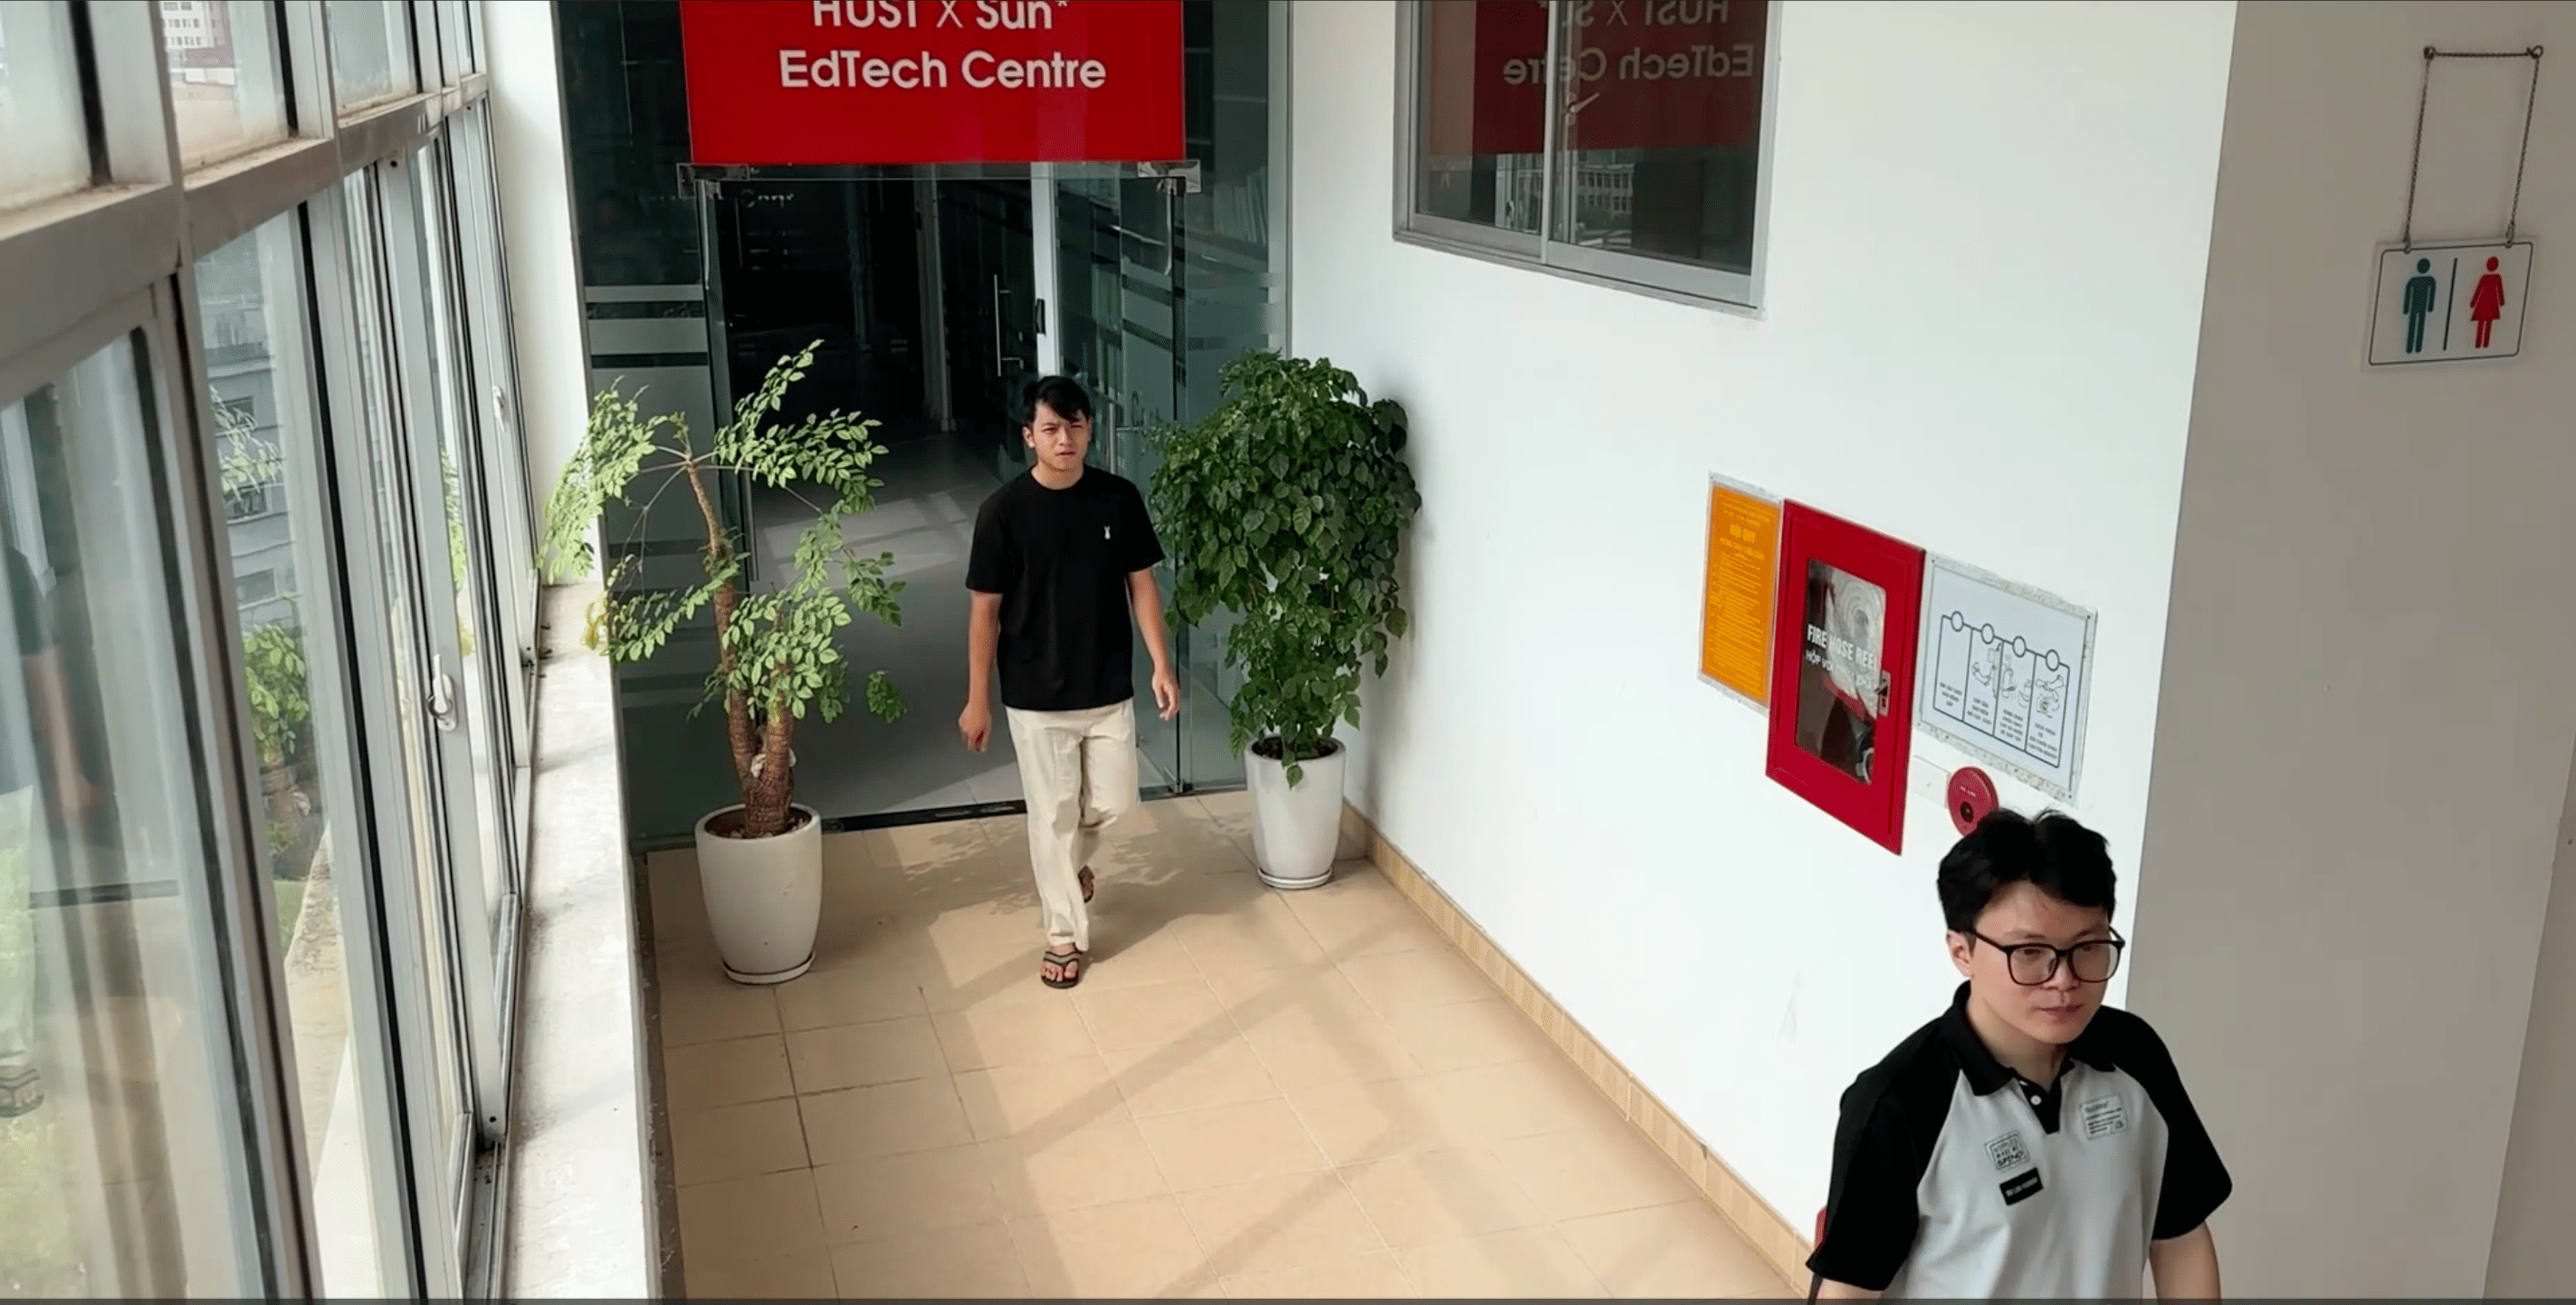
\includegraphics[width=\textwidth]{Figure/edtech_high.png}
        \caption{High altitude view}
        \label{fig:edtech_high1}
    \end{subfigure}
    \hfill
    \begin{subfigure}[b]{0.48\textwidth}
        \centering
        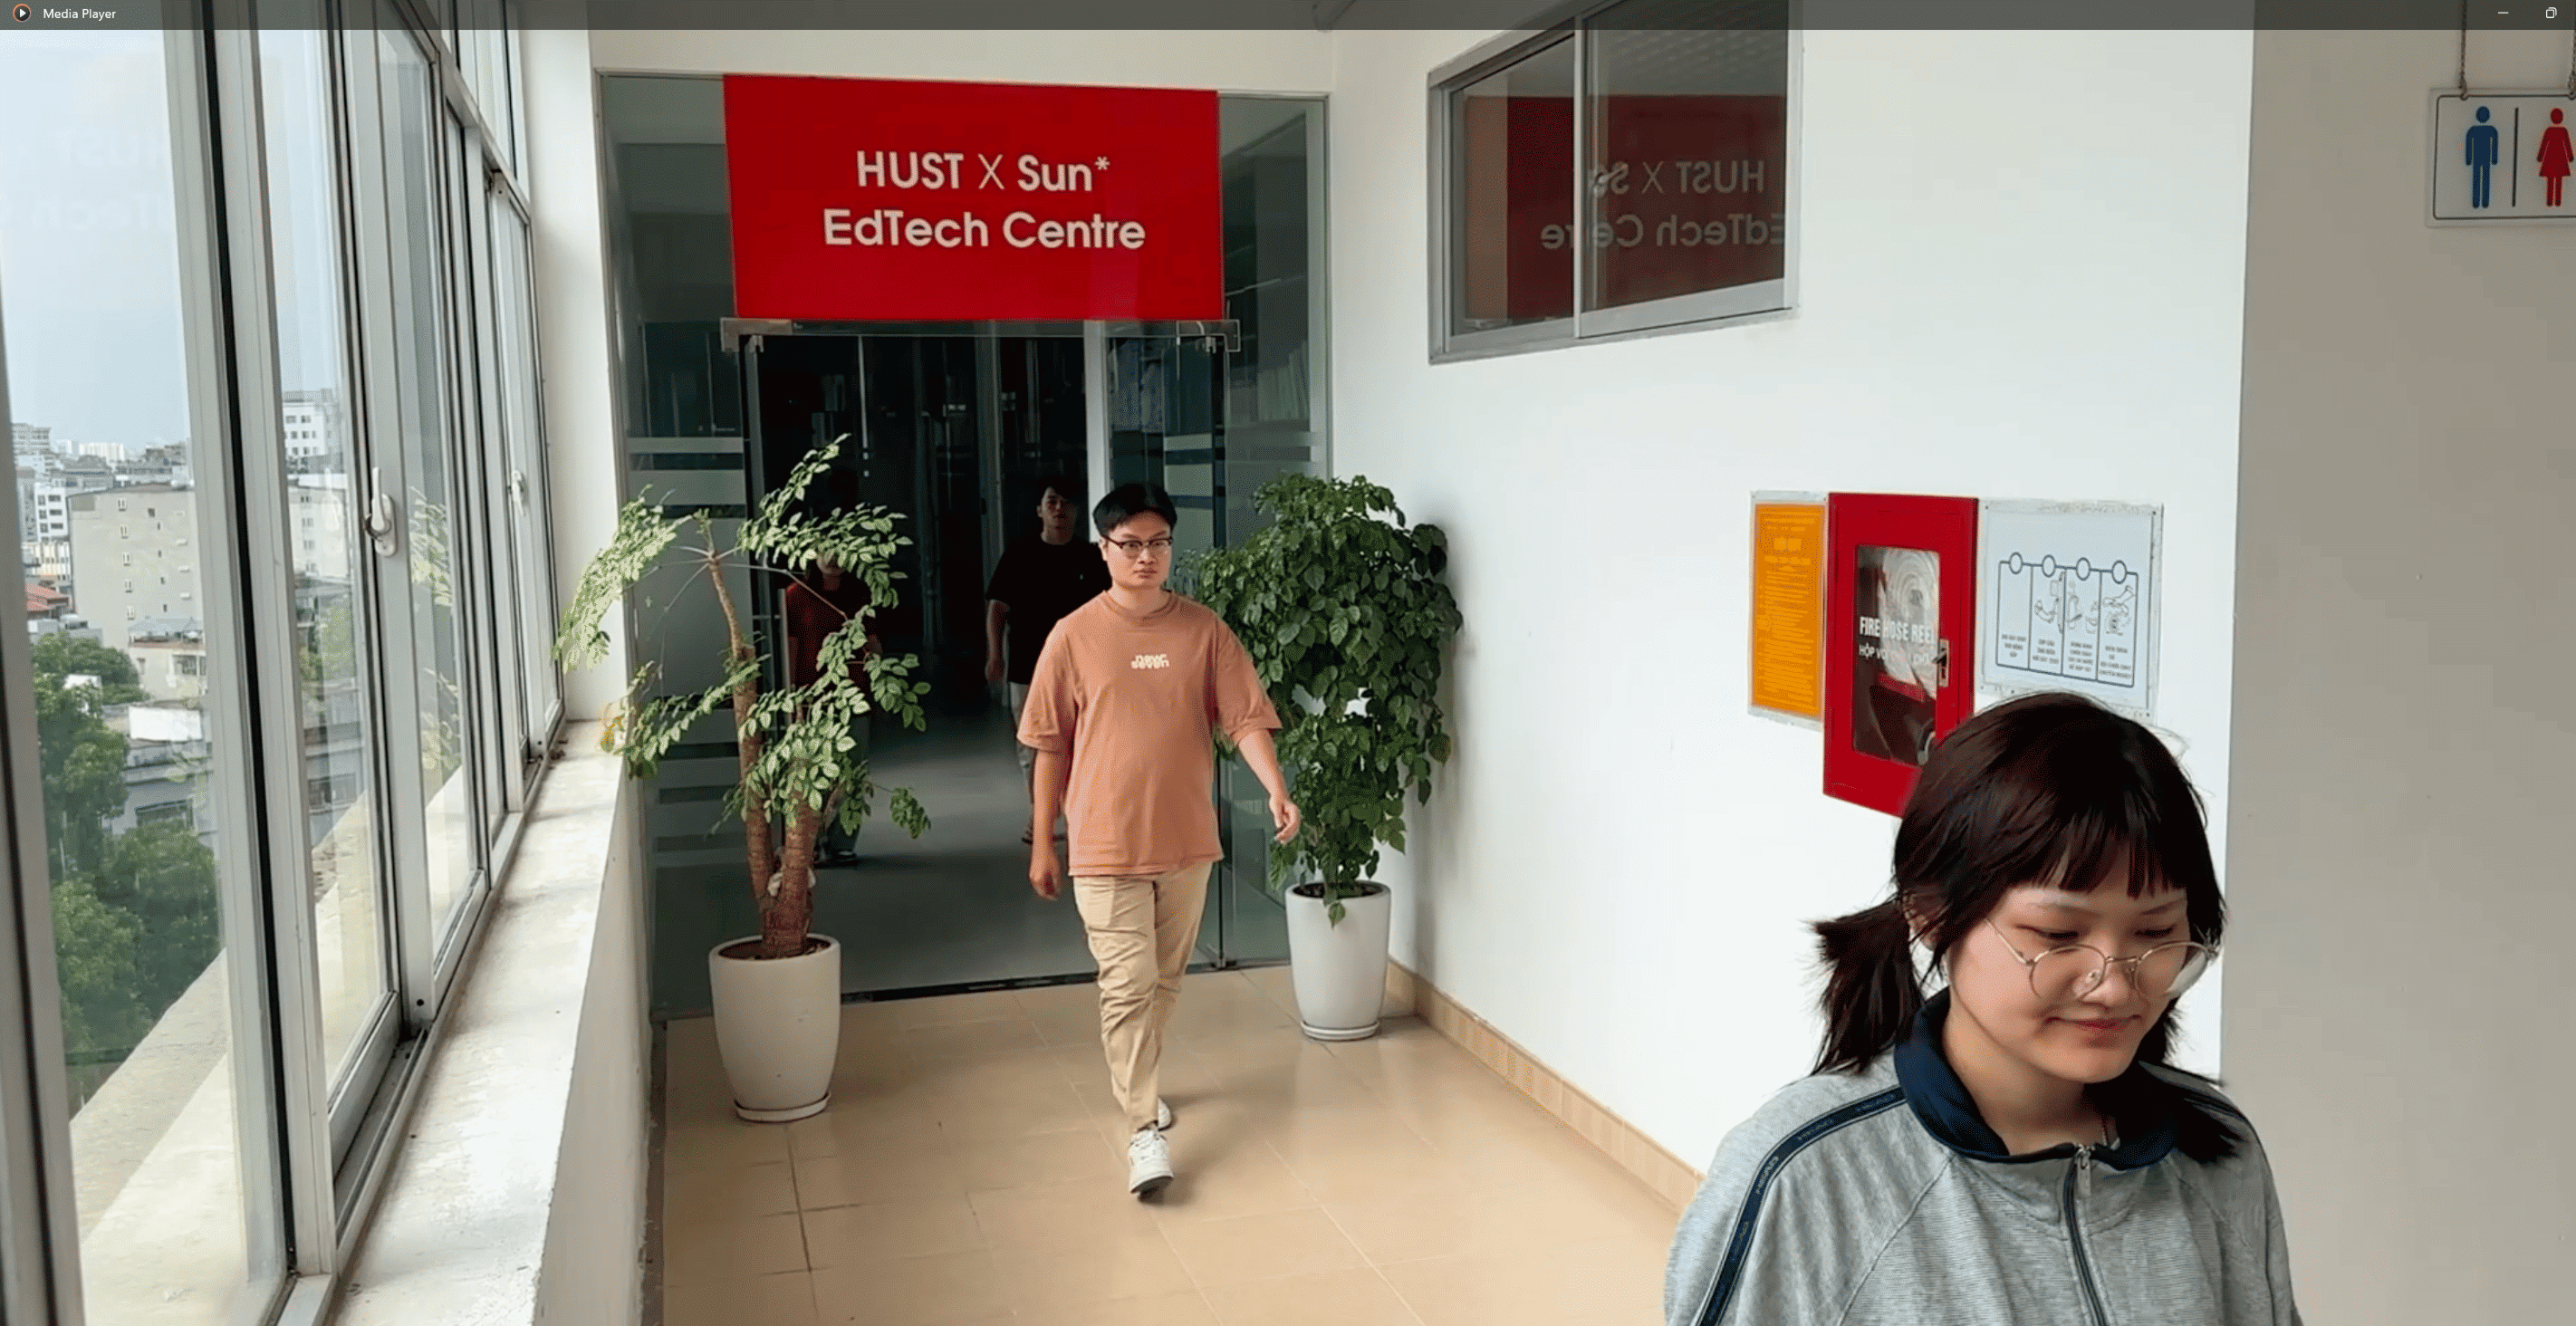
\includegraphics[width=\textwidth]{Figure/edtech_low.png}
        \caption{Low altitude view}
        \label{fig:edtech_low1}
    \end{subfigure}
    \caption{First pair of BK6I dataset samples showing different altitude perspectives}
    \label{fig:bk6i_pair1}
\end{figure}

\begin{figure}[htbp]
    \centering
    \begin{subfigure}[b]{0.48\textwidth}
        \centering
        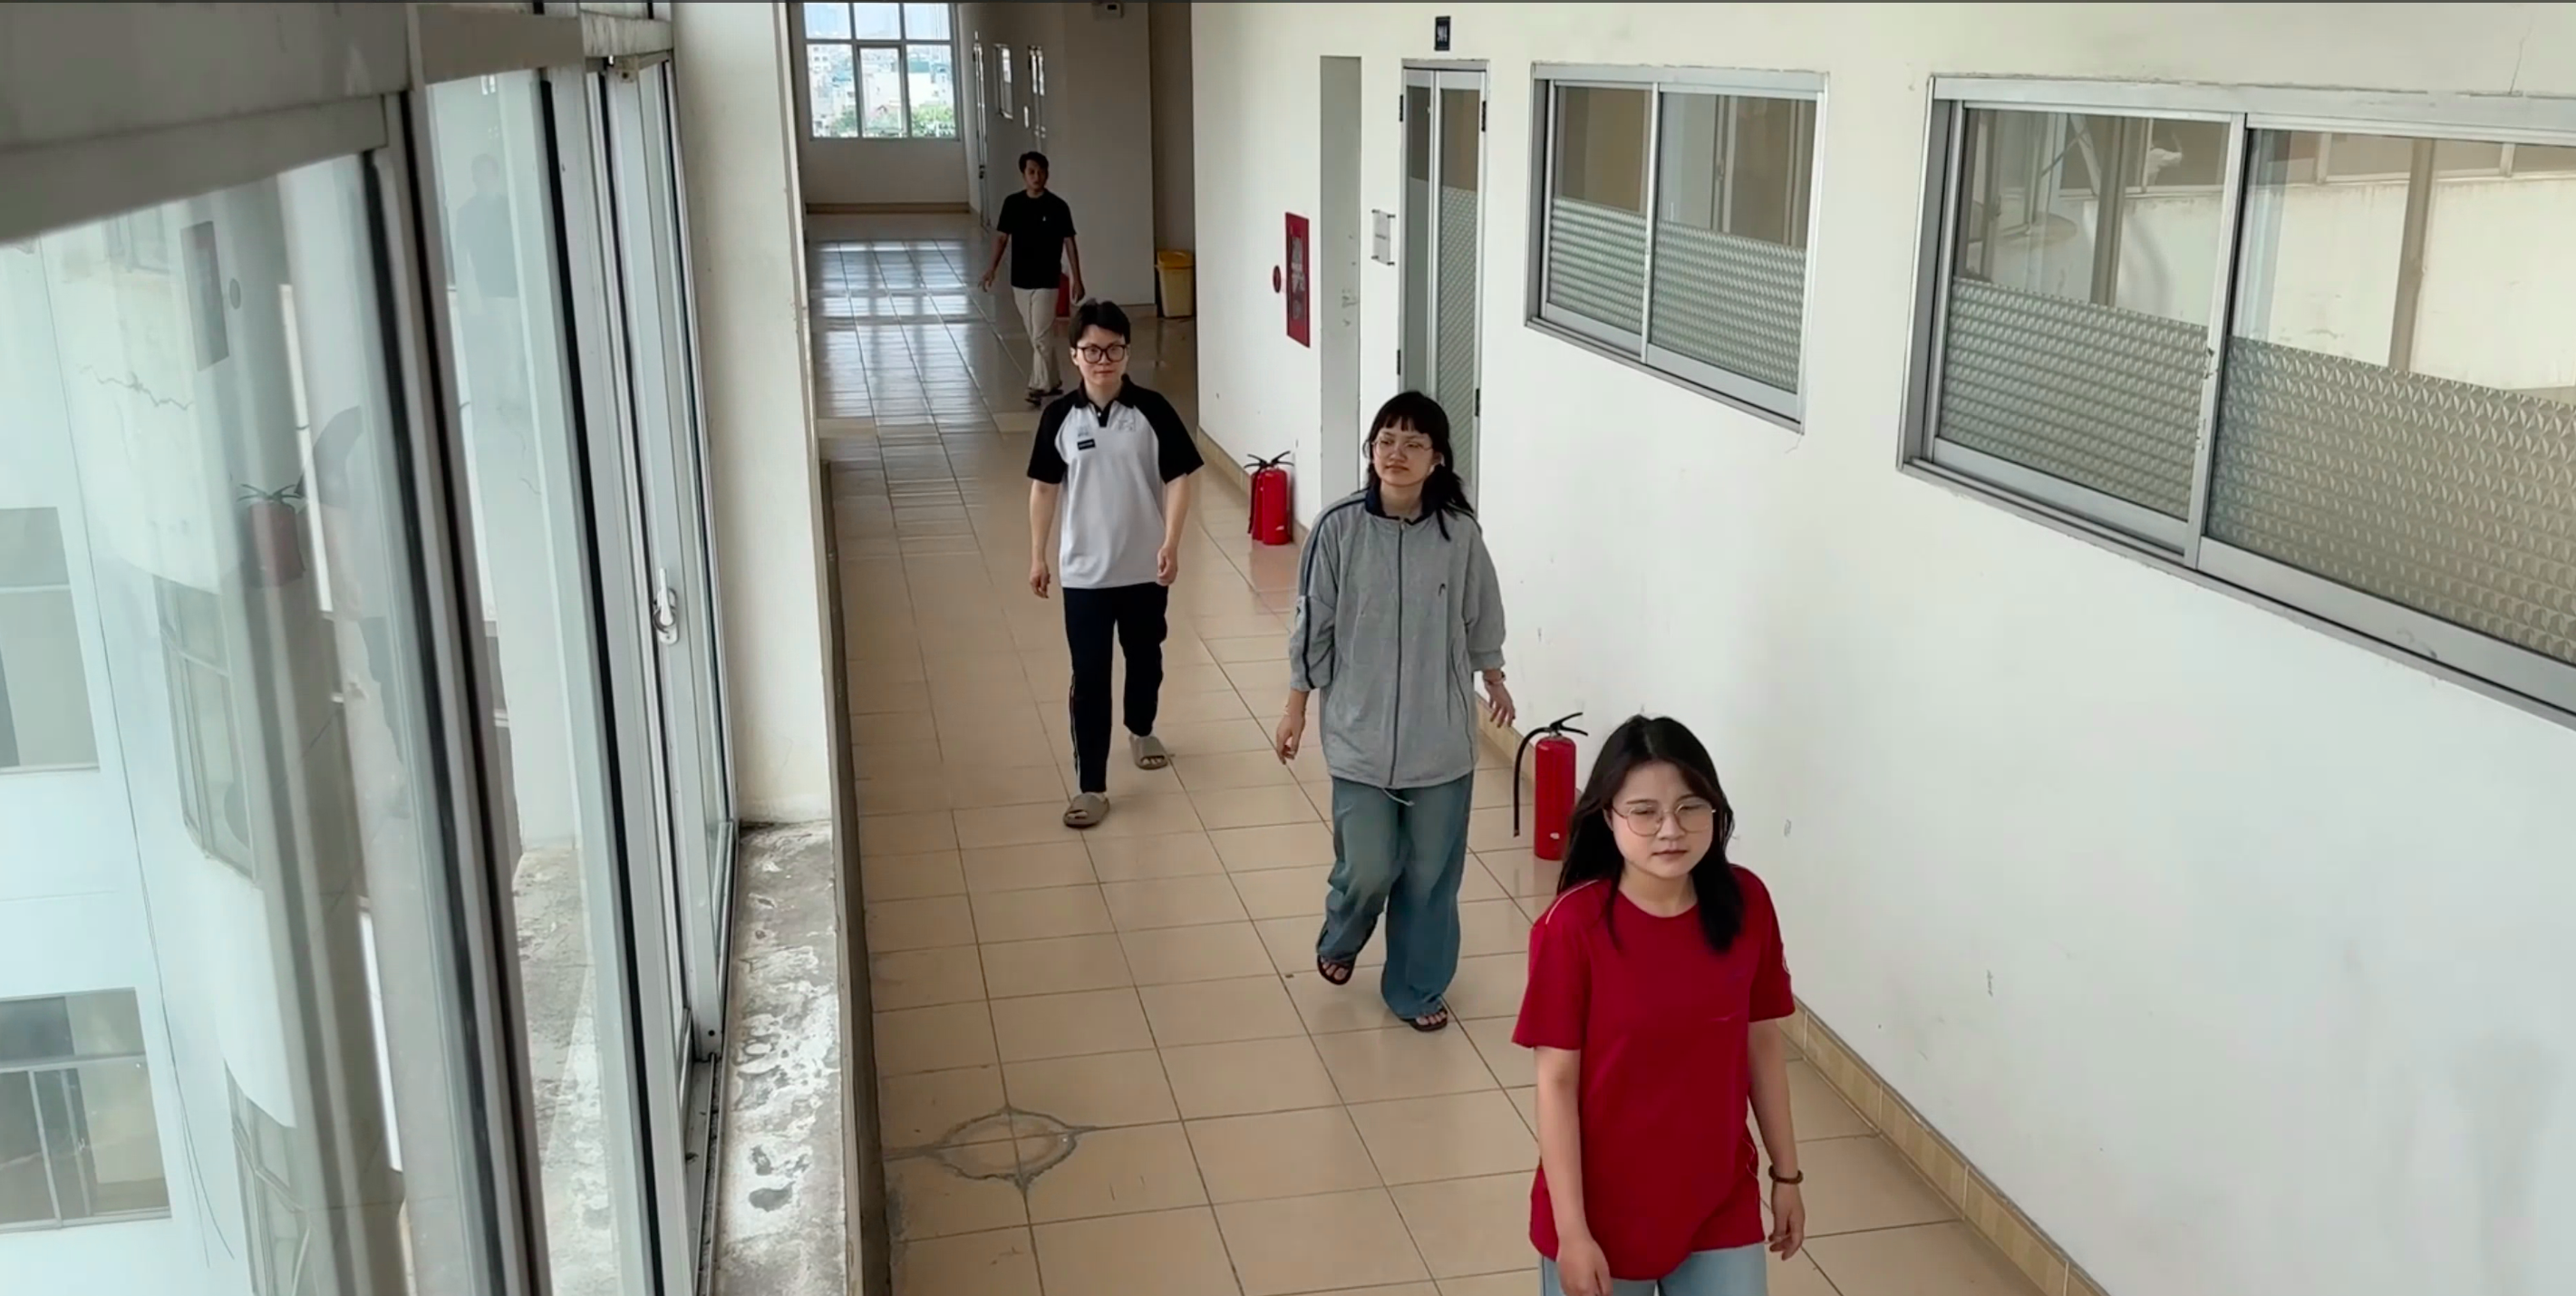
\includegraphics[width=\textwidth]{Figure/edtech_high_2.png}
        \caption{High altitude view}
        \label{fig:edtech_high2}
    \end{subfigure}
    \hfill
    \begin{subfigure}[b]{0.48\textwidth}
        \centering
        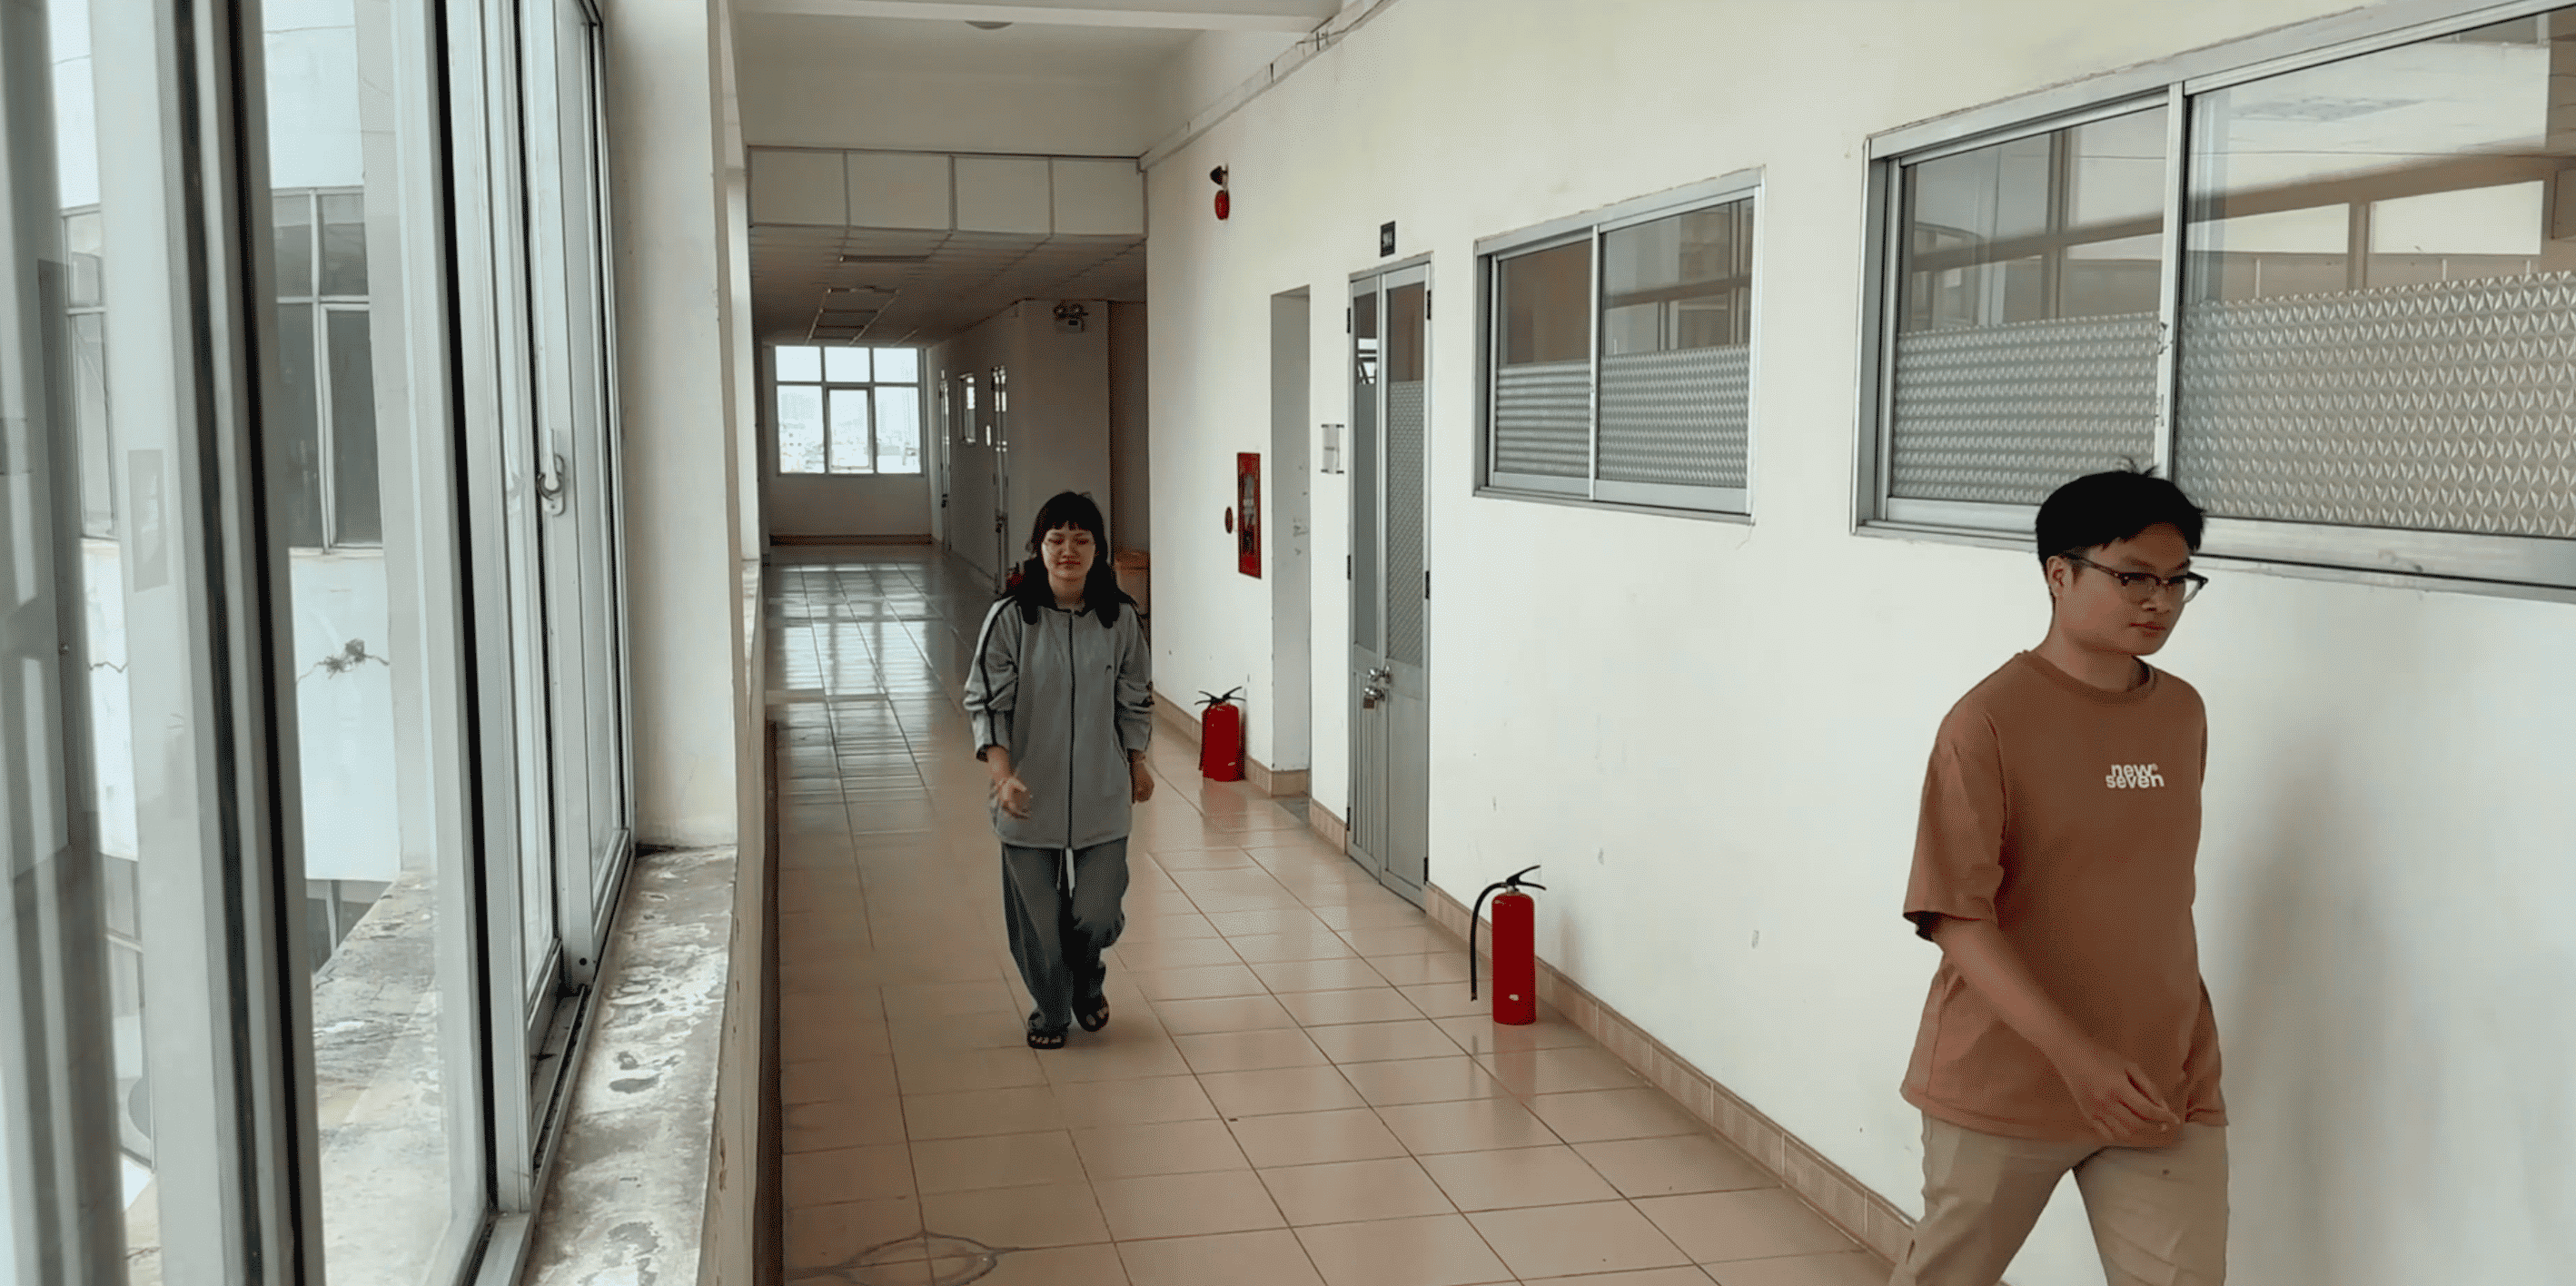
\includegraphics[width=\textwidth]{Figure/edtech_low_2.png}
        \caption{Low altitude view}
        \label{fig:edtech_low2}
    \end{subfigure}
    \caption{Second pair of BK6I dataset samples showing different altitude perspectives}
    \label{fig:bk6i_pair2}
\end{figure}

\begin{figure}[htbp]
    \centering
    \begin{subfigure}[b]{0.48\textwidth}
        \centering
        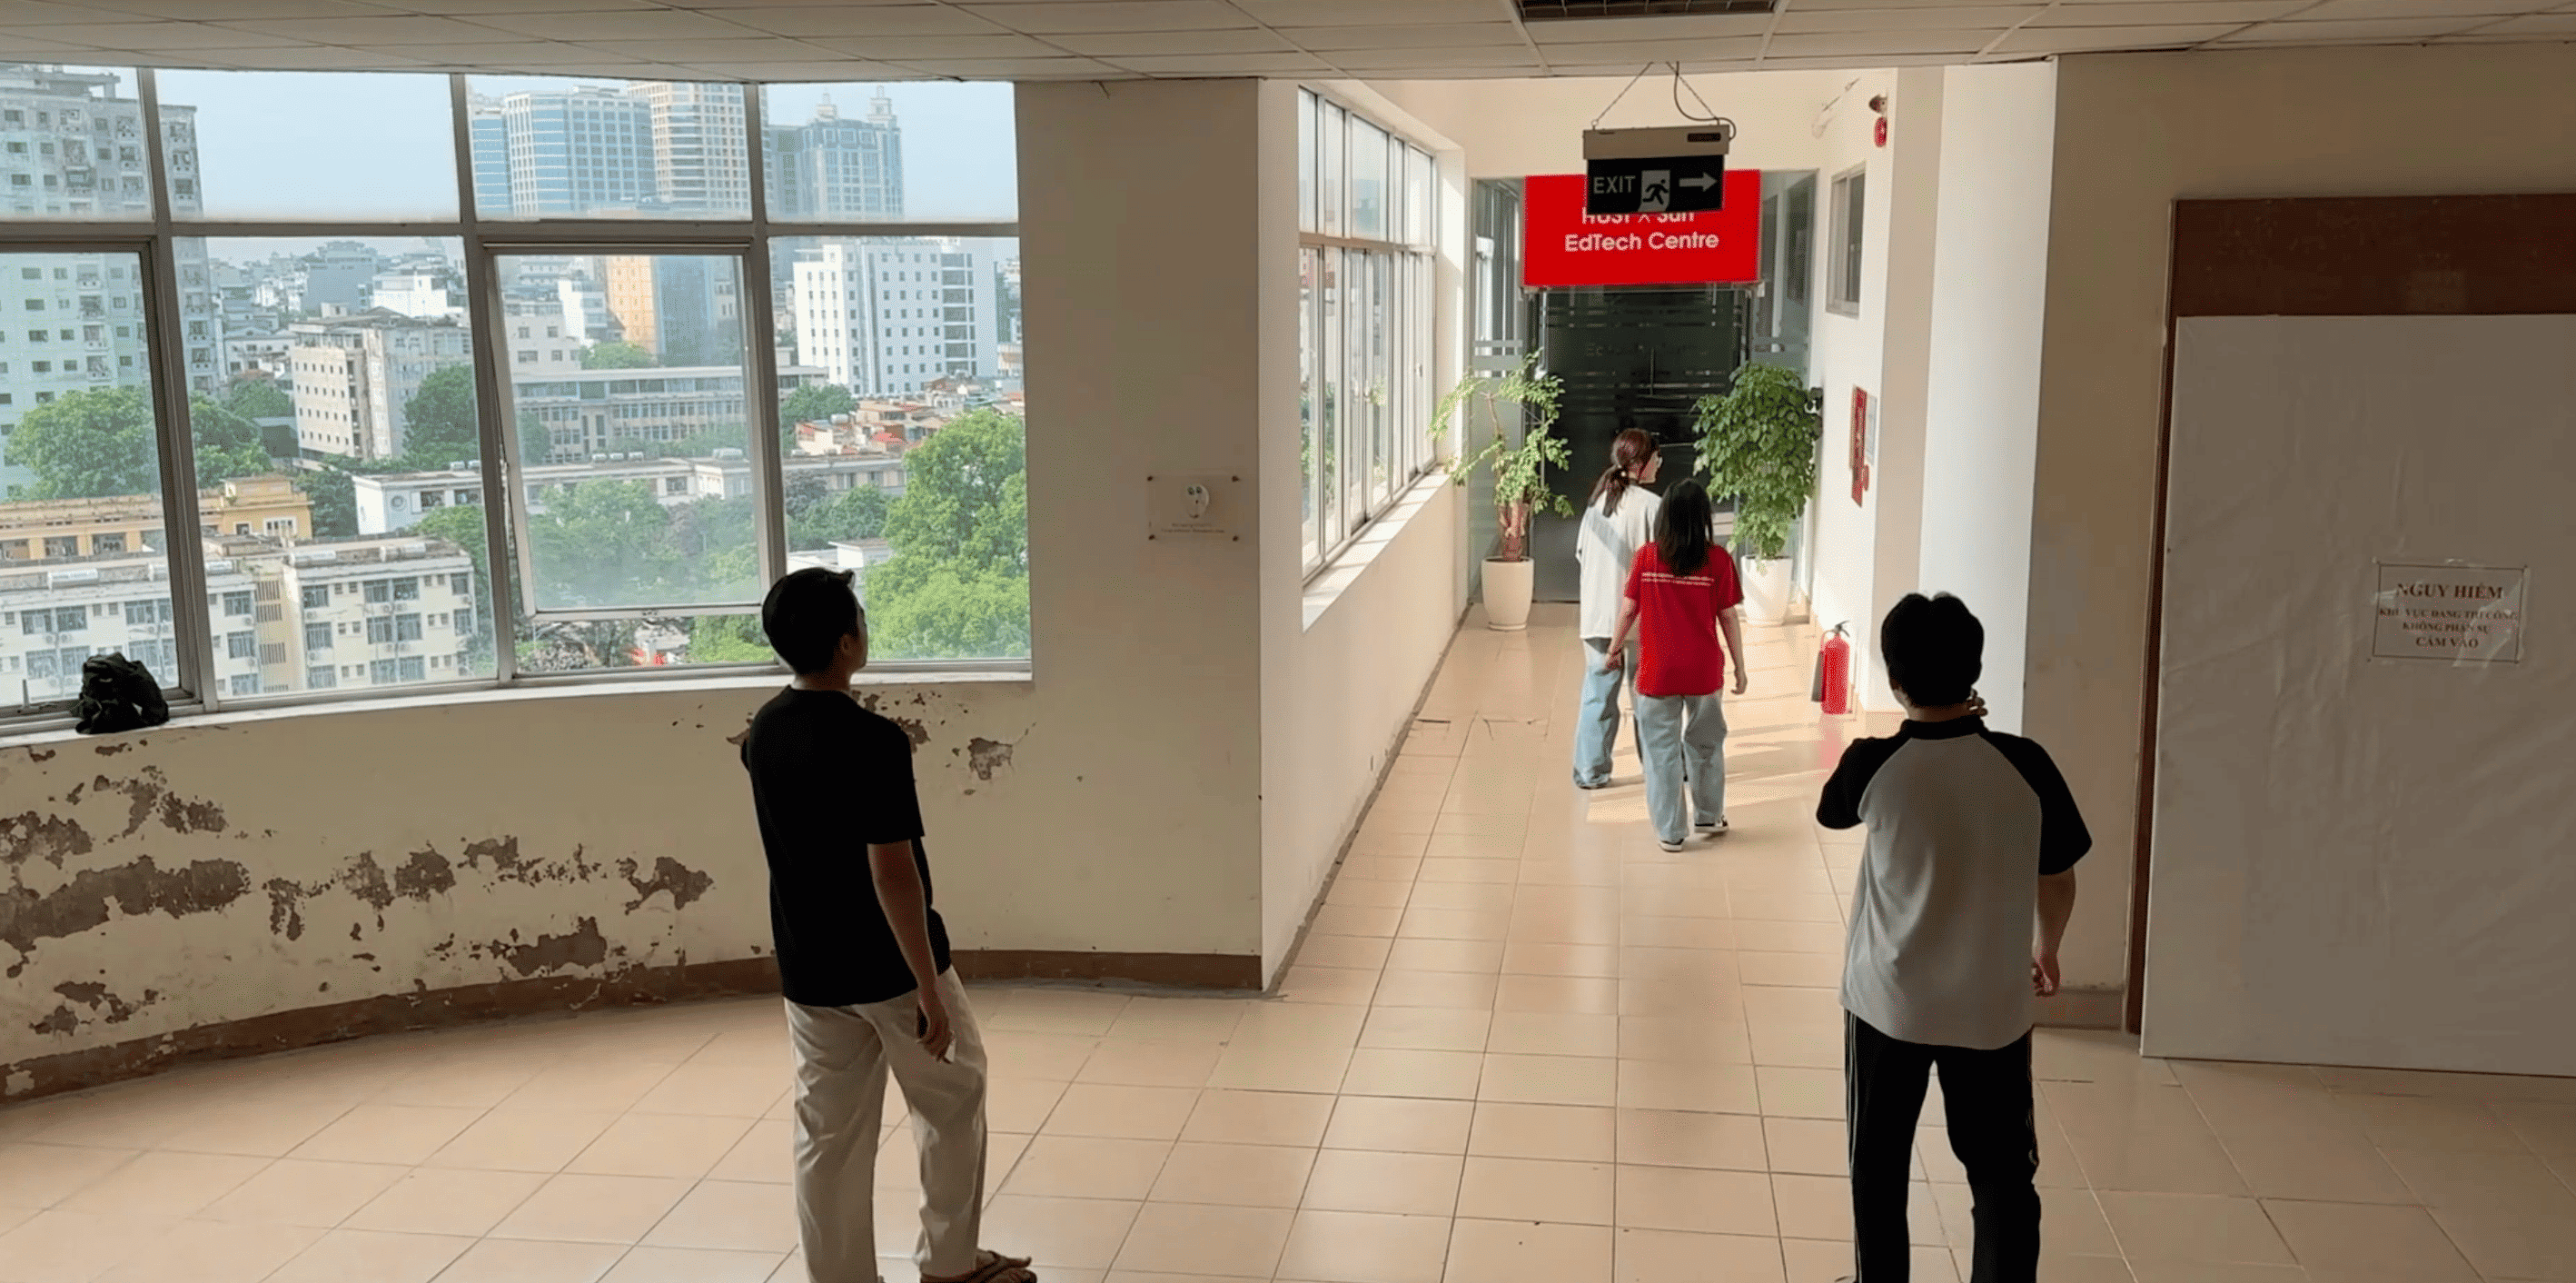
\includegraphics[width=\textwidth]{Figure/overlap_1.png}
        \caption{Overlap view from first camera}
        \label{fig:overlap1}
    \end{subfigure}
    \hfill
    \begin{subfigure}[b]{0.48\textwidth}
        \centering
        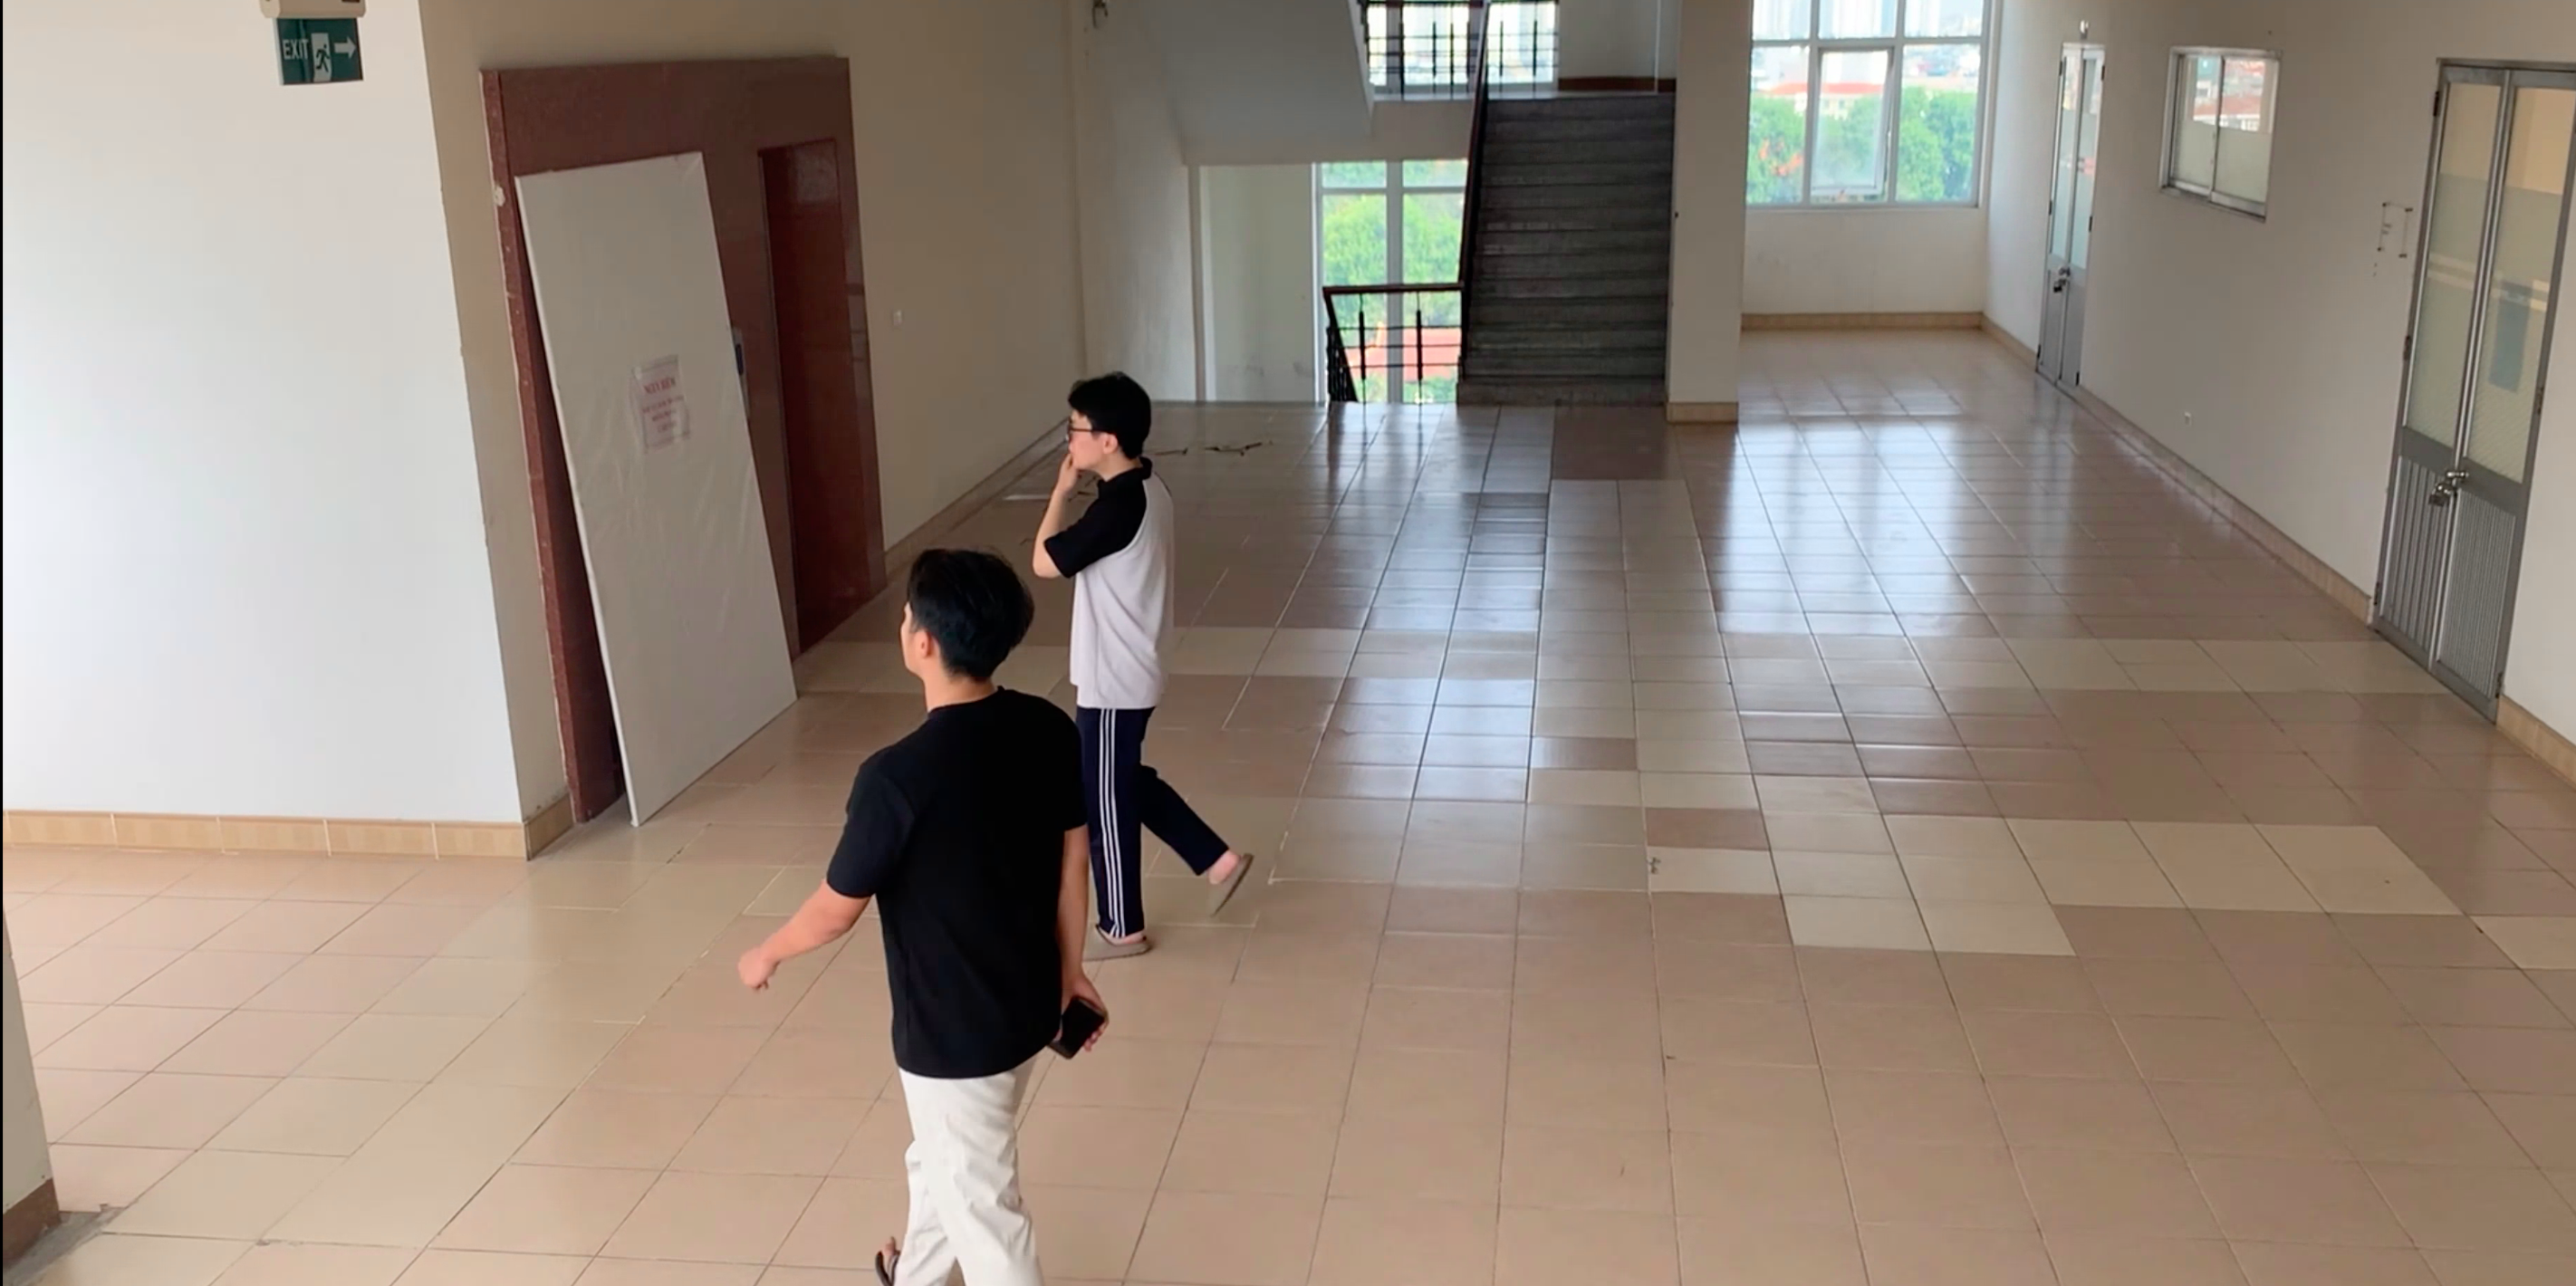
\includegraphics[width=\textwidth]{Figure/overlap_2.png}
        \caption{Overlap view 2}
        \label{fig:overlap2}
    \end{subfigure}
    \caption{Overlap view of BK6I dataset recorded from two different cameras with different angle and lighting conditions}
    \label{fig:overlap}
\end{figure}




\section{Result for detection model}
\label{sec:detection_experiments}
The performance of the detection module on edge devices was assessed using three different methods. The first involved running the module in its native PyTorch environment, while the second tested it after conversion to ONNX, finally the third tested it after conversion to OpenVINO. The module processed all images to generate an initial output before applying NMS to remove redundant bounding boxes and refine the final detections. Performance metrics were computed after applying NMS. In both cases, NMS's IoU threshold was set to 0.45, and the confidence threshold was 0.25. Consequently, only bounding boxes with a confidence score of at least 0.25 were considered, and two boxes were classified as overlapping if their IoU value was 0.45 or higher.

The metrics for evaluating the performance of edge devices are:

\begin{itemize}
    \item \textbf{AP@0.5}: Measures the precision of object detection predictions at an Intersection over the Union threshold of 0.5.
    \item \textbf{mAP}: Calculates the average precision across all classes and IoU thresholds, reflecting overall detection accuracy.
    \item \textbf{FPS}: Represents the inference speed, showing how many frames the model processes per second.
\end{itemize}

\begin{table}[h]
\centering
\caption{Results of Detection Module}
\label{tab:detection_results}
\begin{tabular}{|l|c|c|c|}
\hline
\textbf{Model} & \textbf{AP@0.5} & \textbf{mAP} & \textbf{FPS} \\
\hline
YOLOv8n & 0.9158 & 0.7831 & 10.8 \\
\hline
YOLOv10n & 0.9477 & 0.8157 & 11.4 \\
\hline
YOLOv11n & 0.9521 & 0.8203 & 12.1 \\
\hline
\end{tabular}
\end{table}

The metrics for evaluating model architecture:

\begin{itemize}
    \item \textbf{Params (M)}: The total number of model parameters (in millions), indicating memory requirements.
    \item \textbf{FLOPS (B)}: The number of floating-point operations (in billions) required during inference, reflecting computational efficiency.
\end{itemize}

\begin{table}[h]
\centering
\caption{Computational complexity in comparison}
\label{tab:computational_complexity}
\begin{tabular}{|l|c|c|}
\hline
\textbf{Model} & \textbf{Params (M)} & \textbf{FLOPS (B)} \\
\hline
YOLOv8n & 3.1 & 8.8 \\
\hline
YOLOv10n & 2.7 & 8.7 \\
\hline
YOLOv11n & 2.6 & 6.5 \\
\hline
\end{tabular}
\end{table}

YOLOv11n was selected for our detection module based on its superior balance of accuracy and efficiency. Compared to YOLOv8n, YOLOv11n achieved higher detection performance (AP@0.5 of 0.9521 vs. 0.9158, and mAP of 0.8203 vs. 0.7831) while demonstrating competitive inference speed (12.1 FPS vs. 10.8 FPS). More importantly, YOLOv11n requires significantly fewer computational resources with 16.1\% fewer parameters (2.6M vs. 3.1M) and 26.1\% fewer FLOPS (6.5B vs. 8.8B). When compared to YOLOv10n, YOLOv11n shows marginal improvements in accuracy metrics (AP@0.5: 0.9521 vs. 0.9477, mAP: 0.8203 vs. 0.8157) with slightly higher throughput (12.1 FPS vs. 11.4 FPS) and reduced computational complexity (2.6M vs. 2.7M parameters). This combination of the highest accuracy metrics, competitive inference speed, and the lowest computational demands makes YOLOv11n the optimal choice for our resource-constrained person re-identification system, ensuring reliable detection performance while maintaining practical deployability on edge devices with severe hardware limitations.

\begin{table}[h]
\centering
\caption{YOLOv11n performance comparison across model formats and CPU configurations}
\label{tab:yolov11n_performance}
\begin{tabular}{|l|c|c|c|c|c|c|}
\hline
\multirow{2}{*}{\textbf{Format}} & \multicolumn{3}{c|}{\textbf{1 core CPU}} & \multicolumn{3}{c|}{\textbf{4 cores CPU}} \\
\cline{2-7}
 & \textbf{FPS} & \textbf{CPU (\%)} & \textbf{RAM (MB)} & \textbf{FPS} & \textbf{CPU (\%)} & \textbf{RAM (MB)} \\
\hline
.pt & 12.1 & 99.7 & 312 & 11.8 & 26 & 315 \\
\hline
ONNX & 9 & 99.8 & 352 & 10.5 & 94 & 355 \\
\hline
OpenVINO & 9.2 & 99.6 & 388 & 10.2 & 93 & 385 \\
\hline
\end{tabular}
\end{table}

The performance analysis reveals important trade-offs between different model formats in resource-constrained environments. While OpenVINO achieved moderate FPS (9.2) among single-core configurations, it consumed significantly more memory (388 MB) and maintained near-maximum CPU utilization (99.6\%). Similarly, ONNX format showed comparable performance (9.0 FPS) but with even higher memory consumption (352 MB) and maximum CPU usage (99.8\%). In contrast, the native PyTorch (.pt) format demonstrated the most balanced resource utilization, achieving superior FPS performance (12.1) with 312 MB RAM consumption and 99.7\% CPU usage on single-core configurations.

For CPU-based device with severe constraints with 1 CPU core and 512 MB RAM, the native PyTorch format proves most suitable despite its lack of optimization features. While ONNX and OpenVINO formats support multi-core utilization for potential speedup, their resource overhead in single-core scenarios outweighs their performance benefits. The .pt format's superior FPS performance (12.1 vs. 9.2 for OpenVINO) combined with lower memory footprint makes it the optimal choice for deployment on edge devices where resource efficiency is more critical than absolute computational optimization.


\section{Result for embedding models}
\label{sec:embedding_experiments}
This experiment evaluates lightweight feature extraction models for person Re-ID using internally created video data. The primary objective is identifying models that achieve optimal accuracy-efficiency trade-offs suitable for deployment in resource-constrained environments requiring fast inference.

We focused on lightweight architectures, particularly OSNet and LightMBN, designed for efficient feature extraction while maintaining high discriminative power. These models were evaluated on their ability to generate meaningful embeddings from video frames and accurately retrieve correct identities across different appearances. Additionally, we compared lightweight models against SOTA Re-ID models to analyze performance-computational cost trade-offs, particularly inference speed.

The emphasis on lightweight models addresses the need for Re-ID deployment on edge devices with limited computational resources and real-time processing requirements. Traditional high-accuracy Re-ID models often demand significant computational power, making them impractical for such environments.

Table presents a comprehensive performance comparison of various ReID models on the CUHK03-D dataset. OSNet demonstrates an exceptional balance between computational efficiency and performance, achieving competitive mAP (63.4\%) and Rank-1 accuracy (65.2\%) with only 2.2 million parameters.

\begin{table}[ht]
\centering
\caption{Performance comparison of models on CUHK03-D dataset}
\begin{tabular}{|c|c|c|c|}
\hline
\textbf{Model} & \textbf{mAP (\%)} & \textbf{R-1 (\%)} & \textbf{Params (Million)} \\ 
\hline
OSNet \cite{zhou2019omniscalefeaturelearningperson} & 63.4 & 65.2 & \textbf{2.2} \\ 
LightMBN \cite{Herzog_2021} & \textbf{82.9} & \textbf{85.9} & 9.0 \\ 
HACNN \cite{li2018harmoniousattentionnetworkperson} & 37.5 & 38.2 & 2.7 \\ 
ResNet50 \cite{he2015deepresiduallearningimage} & 54.7 & 57.3 & 24.5 \\ 
SCSN \cite{Chen_2020_CVPR} & 81.0 & 84.7 & $\sim$26 \\ 
Relation-Net \cite{park2019relationnetworkpersonreidentification} & 69.6 & 74.4 & 43.7 \\ 
RGA-SC \cite{zhang2020relationawareglobalattentionperson} & 74.5 & 79.6 & 27.5 \\ 
HPM \cite{fu2018horizontalpyramidmatchingperson} & 57.5 & 63.9 & 31.9 \\ 
ProNet++ \cite{wang2023rethinkingpersonreidentificationprojectiononprototypes} & 79.1 & 82.6 & $\sim$22 \\ 
NFormer \cite{wang2022nformerrobustpersonreidentification} & 74.7 & 77.3 & $\sim$24 \\ 
\hline
\end{tabular}
\label{tab:cuhk03_comparison}
\end{table}


OSNet's parameter efficiency is remarkable: 81.6\% fewer parameters than LightMBN (9.0M), 91.7\% fewer than ProNet++ ($\sim$22M), and 91.5\% fewer than SCSN ($\sim$26M). While LightMBN achieves superior accuracy metrics (82.9\% mAP, 85.9\% R-1), OSNet delivers 73.1\% of LightMBN's mAP and 75.9\% of its Rank-1 accuracy using only 24.4\% of the parameters.

Compared to HACNN with similar parameter count (2.7M), OSNet demonstrates substantially better performance with 25.9 and 27.0 percentage point advantages in mAP and Rank-1 accuracy, respectively. Against ResNet50 (24.5M parameters), OSNet maintains competitive 63.4\% mAP while using just 9.0\% of the parameters.

Given these findings, OSNet was chosen for the thesis implementation because of its outstanding balance between computational efficiency and performance metrics. This model is particularly well-suited for deployment on edge devices with limited resources, where reducing computational demands is essential while preserving sufficient Re-ID performance for real-time processing requirements.

\section{Result for gender classification}
\label{sec:classification_experiments}
\input{Chapter/4_4_Gender}

\section{Ray Serve Performance}
\label{sec:ray_serve_performance}




\end{document}